\begin{problem}{텐트}
	{standard input}{standard output}
	{2초}{512MB}{}
	
	JOI 군은 캠프장을 운영하고 있다. 이 캠프장은 $H$ 행 $W$ 열로 나뉘어 있다. 캠프장의 세로 방향은 남북 방향으로, 가로 방향은 동서 방향으로 놓여있다. 북쪽에서 $i$ 번째 행, 서쪽에서 $j$ 번째 열에 ($1 \le i \le H$, $1 \le j \le W$) 있는 구획을 $(i, j)$번 구획이라고 쓴다.
	
	JOI 군은 몇몇 구획에 텐트를 배치할 것이다. 각 텐트는 정확히 하나의 구획을 차지해야 한다. 하나의 구획에 두 개 이상의 텐트가 있을 수 없다.
	
	각 텐트는 동서남북 중 한 방향에 입구가 있다. 텐트의 입구 방향은 다음 조건을 만족해야 한다.
	
	\begin{itemize}
		\item 만약 $(i_1, j)$번 구획과 $(i_2, j)$번 구획에 ($1 \le i_1 < i_2 \le H$, $1 \le j \le W$) 모두 텐트가 놓여 있으면, $(i_1, j)$번 구획에 있는 텐트의 입구 방향은 남쪽으로, $(i_2, j)$번 구획에 있는 텐트의 입구 방향은 북쪽으로 놓여있어야 한다.
		\item 만약 $(i, j_1)$번 구획과 $(i, j_2)$번 구획에 ($1 \le i \le H$, $1 \le j_1 < j_2 \le W$) 모두 텐트가 놓여 있으면, $(i, j_1)$번 구획에 있는 텐트의 입구 방향은 동쪽으로, $(i, j_2)$번 구획에 있는 텐트의 입구 방향은 서쪽으로 놓여있어야 한다.
	\end{itemize}

	JOI 군이 캠프장에 위와 같은 조건을 만족하도록 적어도 하나의 텐트를 배치하는 경우의 수를 알고 싶다. 어떤 구역에 텐트가 배치된 방법이 (텐트가 배치되어 있는지와 텐트의 입구 방향) 다르면, 텐트를 배치하는 두 방법은 서로 다른 방법이다.
	
	문제의 조건을 만족하도록 적어도 하나의 텐트를 배치하는 방법의 수를 1 000 000 007로 나눈 나머지를 출력하여라.
	
	
	\InputFile
	
	표준 입력에서 다음 입력이 주어진다.
	
	\begin{itemize}
		\item 첫째 줄에는 두 개의 정수 $H$, $W$가 공백으로 구분되어 주어진다. 이는 JOI 군이 운영하는 캠프장이 $H$ 행 $W$ 열로 이루어져 있다는 것을 의미한다.
	\end{itemize}
		
	\OutputFile
	
	문제의 조건을 만족하도록 캠프장에 적어도 하나의 텐트를 배치하는 방법의 수를 1 000 000 007로 나눈 나머지를 출력하여라.
	
	
	\Constraints
	
	\begin{itemize}
		\item $1 \le H \le 3\ 000$.
		\item $1 \le W \le 3\ 000$.
	\end{itemize}
	
	
	\SubtaskWithCost{1}{48}
	\begin{itemize}
		\item $1 \le H \le 300$.
		\item $1 \le W \le 300$.
	\end{itemize}

	
	\SubtaskWithCost{2}{52}
	추가 제한조건이 없다.
	
	\Examples
	
	\begin{example}
		\exmp{
			1 2
		}{%
		9
		}%
	\end{example}
	
	동쪽, 서쪽, 남쪽, 북쪽으로 입구가 놓인 텐트를 각각 `\texttt{E}', `\texttt{W}', `\texttt{S}', `\texttt{N}'으로 표현하자. 조건을 만족하도록 텐트를 배치하는 방법은 아래와 같이 9가지가 있다.
	
	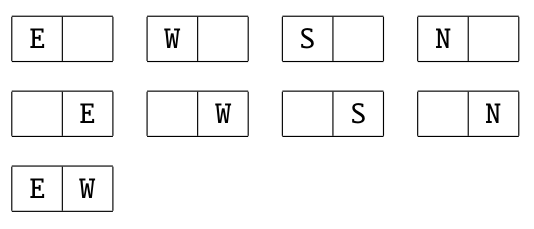
\includegraphics[width=0.35\linewidth]{img1.png}
	
	\begin{example}
		\exmp{
4 3
}{%
3252
}%
		\exmp{
	100 100
}{%
	561068619
}%
	\end{example}
	
	
\end{problem}

